\section{Passive Decomposition}

\begin{frame}
	\frametitle{Passive Decomposition}
	
	\begin{itemize}
		\item First introduced by D. Lee 2008. \footcite{LeePassive}
		\item Proposed system dynamics split:
		\begin{itemize}
			\item Shape	- internal configuration of each robot
			\item Locked - current overall behavior of multiple robot systems 
			\item Coupled - interaction between locked and shape dynamics
		\end{itemize}
		\item Passive decomposition
		\begin{itemize}
			\item Applying a control law to cancel the dynamics coupling terms without energy generation
			\item Enforces energetic passivity
		\end{itemize}
	\end{itemize}
\end{frame}

\begin{frame}
	\frametitle{Passive Decomposition - QM systems \footcite{passive-decomp-quadrotor-with-robotic-manip}$\,$  \footcite{decoupled-aerial-manipulation}}
	
	\begin{columns}
		\begin{column}{0.5\textwidth}\centering
			\begin{figure}[H]
				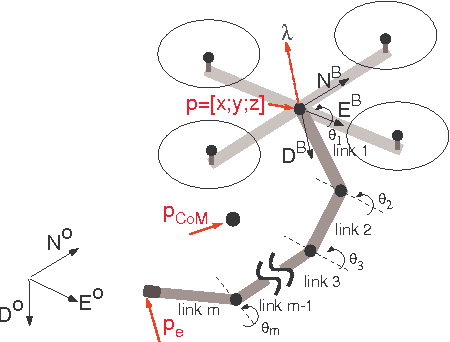
\includegraphics[width=0.9\columnwidth]{figures/aerial_manip.png}	
				\centering
				\caption{QM system${}^{15}$}
				\label{fig:aerial_manip}
			\end{figure}
		\end{column}
		
		\begin{column}{0.5\textwidth}\centering
			\begin{itemize}
			\item Decoupled quadrotor-manipulator(QM) system:
			\begin{itemize}
				\item center-of-mass dynamics in E(3)
				\item Robotic manipulator Lagrange dynamics
			\end{itemize}
			\item End-effector control law:
			\begin{itemize}
				\item Backstepping-like $\text{controller}^{15}$
				\item PID $\text{cascade}^{16}$
			\end{itemize}
			\end{itemize}
		\end{column}
	\end{columns}
 \end{frame}

\begin{frame}
	\frametitle{Passivity Based Control - Payload Transportation}
	\begin{itemize}
		\item C. Meissen et al. 2017. \footcite{passivity-based-formation-load} - General formation and internal control laws
		\item M E. Guerrero et al. 2015. \footcite{passivity-based-payload-minimum-swing} - An Interconnection and Damping Assignment - Passivity Based Control (IDA-PBC) for payload swing suppression
		\item P. Prajapati et al. 2019. \footcite{payload-and-human} - Master-slave transportation strategy with human-in-the-loop
	\end{itemize}
\end{frame}

\begin{frame}
	\frametitle{Passivity Based Control - Aerial Compliance (1)}
	
	\begin{itemize}
		\item E. Spyrakos et al. 2019. \footcite{passive-variable-impedance-compliant} - Manipulator passivity preservation control (PPC)
		\item Q. Delamare 2019. \footcite{quadrotor-itneraction-environment} - Exploiting physical contact to achieve flight maneuvers
		\item M. Schuster et al. 2019. \footcite{max-wrench-min-energy} - Energy efficient approach to maximum in-flight wrench generation
	\end{itemize}
\end{frame}

\begin{frame}
	\frametitle{Passivity Based Control - Aerial Compliance (2)}
	\begin{itemize}
		\item R. Rashad et al. 2019. \footcite{passivity-based-physical-interaction} - Passivity based control of a fully actuated UAV for aerial physical interaction near hovering by 
	\end{itemize}
	\begin{figure}[H]
		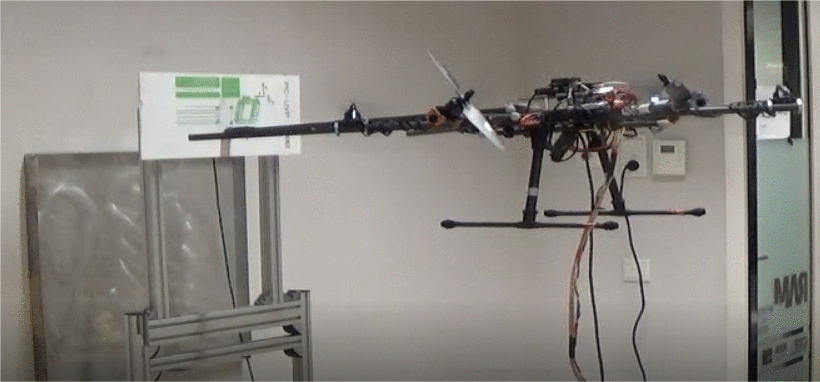
\includegraphics[width=0.6\columnwidth]{figures/passivity-based-interaction.png}	
		\centering
		\caption{A fully-actuated hexarotor UAV applying force to a vertical surface.}
		\label{fig:aerial_compliance}
	\end{figure}
 \end{frame}

\begin{frame}
	\frametitle{Passivity Based Control - Notable Mentions (1)}
	\begin{itemize}
		\item Y. Iarashi et al. 2009. \footcite{passivity-attitude-sync} 
		\begin{itemize}
			\item Passivity based motion coordination of rigid bodies by exchanging information over connected graphs
		\end{itemize} 
		\item H. Yang and D. Lee 2015. \footcite{cooperative-control-quadrotor}
		\begin{itemize}
			\item A hierarchical cooperative control framework
			\item Endowment of a common grasped object with desired behavior (e.g., trajectory tracking, compliant interaction, etc.)
		\end{itemize}
	\end{itemize}
\end{frame}

\begin{frame}
	\frametitle{Passivity Based Control - Notable Mentions (2)}
	\begin{itemize}
		\item P. Robuffo Giordano et al. 2011.\footcite{group-teleoperation} 
		\begin{itemize}
			\item Experimental validation of a decentralized passivity-based control strategy for teleoperating a group UAVs
			\item Master UAV (human-in-the-loop) controls the group motion and receives feedback about the remote slave motion status
		\end{itemize}
		\item D. Lee et al. 2013. \footcite{haptic-teleoperation-uav}
		\begin{itemize}
			\item Semi-autonomous haptic teleoperation control architecture for multiple UAVs
		\end{itemize}
	\end{itemize}
\end{frame}